\section{Implementation}
\label{sec:implementation}

While our proposed API is general and not language specific, we have implemented
\sysname{} prototype in Rust (\textasciitilde 4000 lines of code). \sysname{} is
open source on GitHub.\footnote{\url{https://github.com/awstream/awstream}}
Applications use \sysname{} as a library and configure the execution
mode---profiling, runtime as client, or runtime as server---with command line
arguments.

\begin{table}
  \centering
  \begin{tabular}{c c c c}
    \toprule
    Application & Knobs & Accuracy & Dataset \\
    \midrule
    \specialcell{Augmented\\Reality}
                & \specialcell{resolution \\ frame rate \\ quantization }
                & F1 score~\cite{van1979information}
                & \specialcell{iPhone video clips\\training: office (24
    s)\\testing: home (246 s)} \\
    \midrule
    \specialcell{Pedestrian\\Detection}
                & \specialcell{resolution \\ frame rate \\ quantization }
                & F1 score
                & \specialcell{MOT16~\cite{milan2016mot16}\\training: MOT16-04\\testing: MOT16-03} \\
    \midrule
    \specialcell{Log Analysis\\(Top-K, K=50)}
                & \specialcell{head (N) \\ threshold (T) }
                & \specialcell{Kendall's $\tau$~\cite{abdi2007kendall}}
                & \specialcell{\href{https://www.sec.gov}{SEC.gov} logs~\cite{edgarlog} \\ training: 4 days \\
    testing: 16 days} \\
    \bottomrule
  \end{tabular}
  \caption{Application details.}
  \label{tab:apps}
\end{table}


\begin{figure}
  \centering
  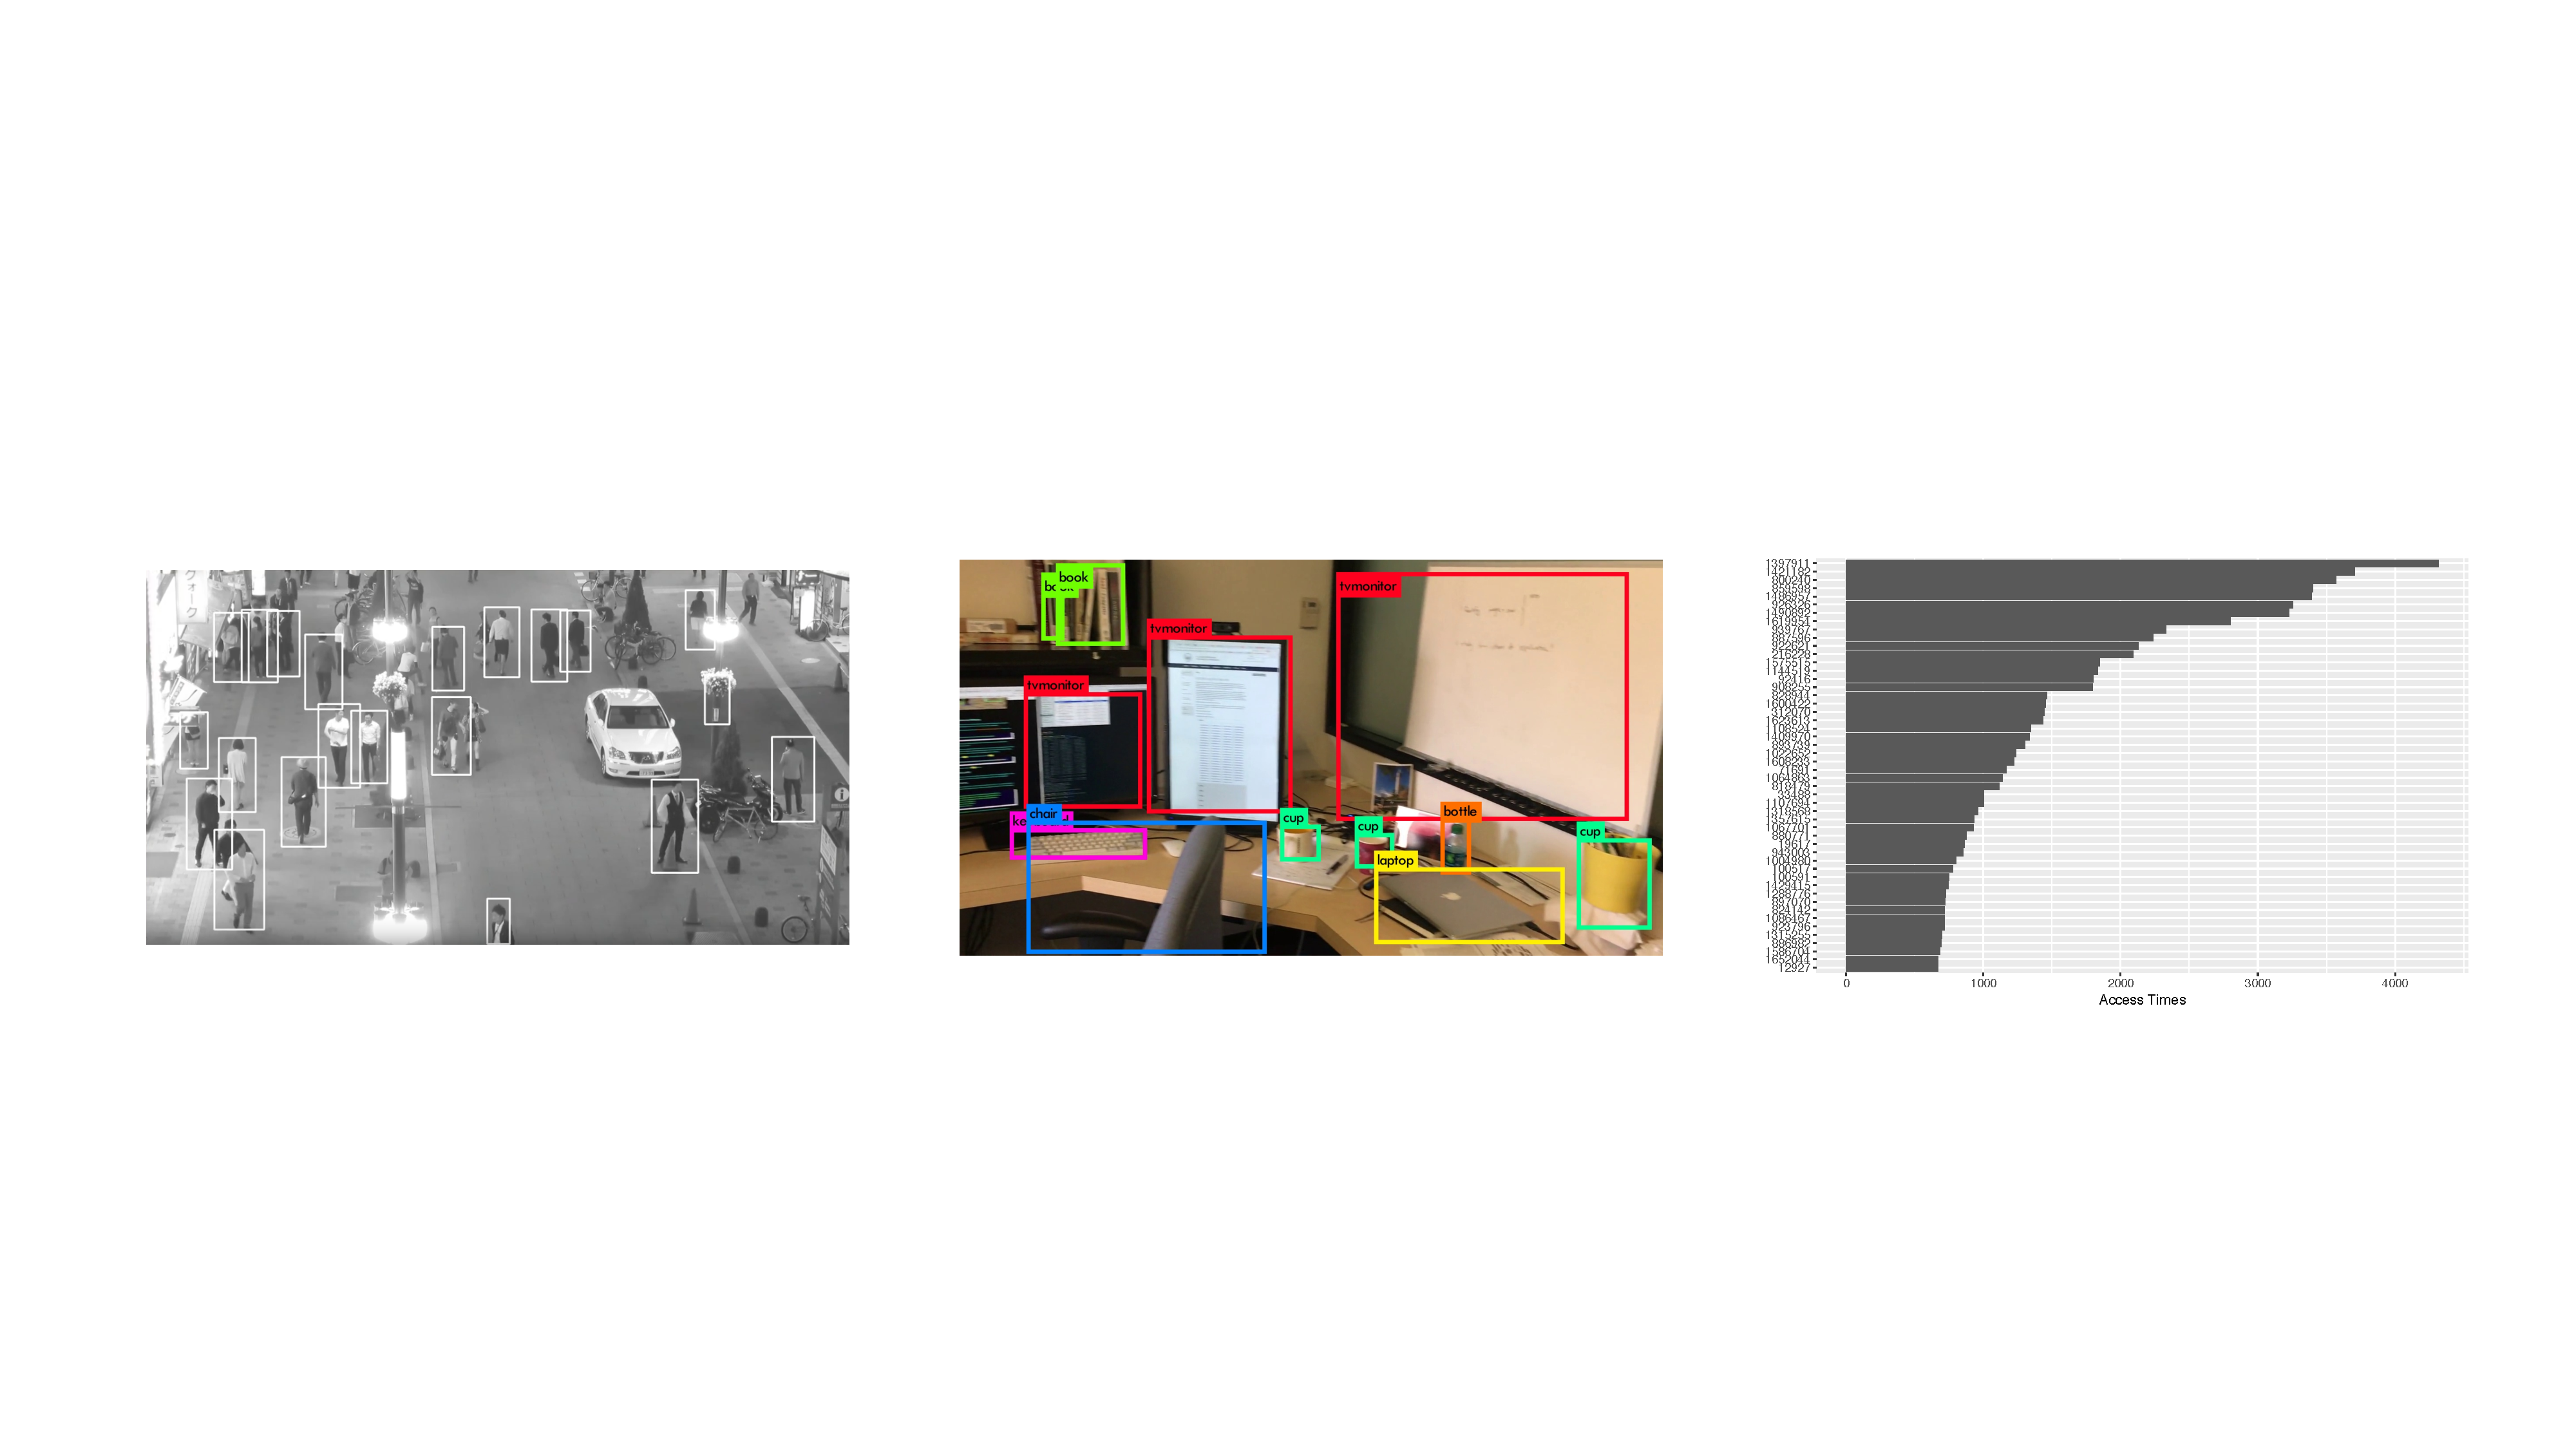
\includegraphics[width=\columnwidth]{figures/apps.pdf}
  \caption{Three \sysname{} applications: augmented reality, pedestrian
    detection, and distributed Top-K.}
  \label{fig:three-apps}
\end{figure}

Using \sysname{}, we have built three applications: augmented reality (AR) that
recognizes nearby objects on mobile phones, pedestrian detection (PD) for
surveillance cameras, and a distributed log analysis to extract the Top-K mostly
accessed files (TK). \autoref{tab:apps} summarizes the application-specific
parts: knobs, accuracy functions, and datasets.

\para{Augmented Reality.} We target at augmented reality applications running on
mobile phones that recognize objects by offloading the heavy computation
elsewhere (e.g.,~the cloud).

Our implementation uses OpenCV~\cite{opencvlibrary} for image-related operations
and YOLO~\cite{darknet13, redmon2016yolo9000}, a GPU-enabled pre-trained neural
network, for object recognition. Videos are encoded with
H.264~\cite{richardson2011h}. Our implementation uses GStreamer~\cite{gstreamer}
with \texttt{x264enc} plugin (\texttt{zerolatency} and constant quality). The
quantization factor affecting encoding quality becomes a knob in addition to
image resolutions and frame rates.

Object recognition returns a list of bounding boxes with the object type. Each
bounding box is a rectangle with normalized coordinates on the image. We compare
the detection against the reference result from raw data, and declare it success
if the intersection over union (IOU) is greater than
50\%~\cite{everingham2010pascal} (illustrated in \autoref{fig:iou}) and the
object type matches. We use F1 score~\cite{van1979information} as the accuracy
function. In terms of dataset, we collected our own video clips: the training
data is a 24-second long video of an office environment; the test data is a
246-second long video of a home environment.

\begin{figure}
  \begin{subfigure}{0.4\textwidth}
    \[
    \text{IOU} = \frac{\text{Area of Intersection}}{\text{Area of Union}}
    \]
  \end{subfigure}%
  \begin{subfigure}{0.2\textwidth}
    \centering
    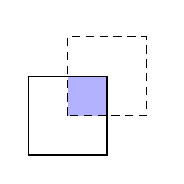
\begin{tikzpicture}
      \fill[color=blue!30] (0.5, 0.5) rectangle (1, 1);
      \node[draw=none] () at (1.5, 1.5) {};
      \draw (0, 0) rectangle (1, 1);
      \draw[densely dashed] (0.5, 0.5) rectangle (1.5, 1.5);
    \end{tikzpicture}
    \caption{IOU=0.14}
  \end{subfigure}%
  \begin{subfigure}{0.2\textwidth}
    \centering
    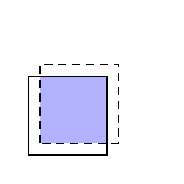
\begin{tikzpicture}
      \fill[color=blue!30] (0.15, 0.15) rectangle (1, 1);
      \node[draw=none] () at (1.5, 1.5) {};
      \draw (0, 0) rectangle (1, 1);
      \draw[densely dashed] (0.15, 0.15) rectangle (1.15, 1.15);
    \end{tikzpicture}
    \caption{IOU=0.57}
  \end{subfigure}%
  \begin{subfigure}{0.2\textwidth}
    \centering
    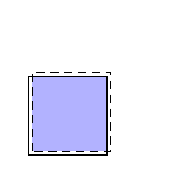
\begin{tikzpicture}
      \fill[color=blue!30] (0.05, 0.05) rectangle (1, 1);
      \node[draw=none] () at (1.5, 1.5) {};
      \draw[densely dashed] (0.05, 0.05) rectangle (1.05, 1.05);
      \draw (0, 0) rectangle (1, 1);
    \end{tikzpicture}
    \caption{IOU=0.82}
  \end{subfigure}
  \caption{Intersection over Union (IOU) illustration.}
  \label{fig:iou}
\end{figure}

%%% Local Variables:
%%% mode: latex
%%% TeX-master: "../network"
%%% End:


\para{Pedestrian Detection.} This application analyzes streams of videos from
installed CCTV cameras and detects pedestrians inside. We use a similar setup
(OpenCV and GStreamer) as our augmented reality application except for the
analytical function. To detect pedestrians, we use GPU-accelerated histogram of
oriented gradients (HOG)~\cite{dalal2005histograms} with the default linear SVM
classifier from OpenCV. Because we do not recognize individual pedestrians, a
successful detection in this case only requires matching the bounding box. Our
evaluation uses MOT16 dataset~\cite{milan2016mot16} for both profiling and
runtime.

\begin{figure}
  \centering
  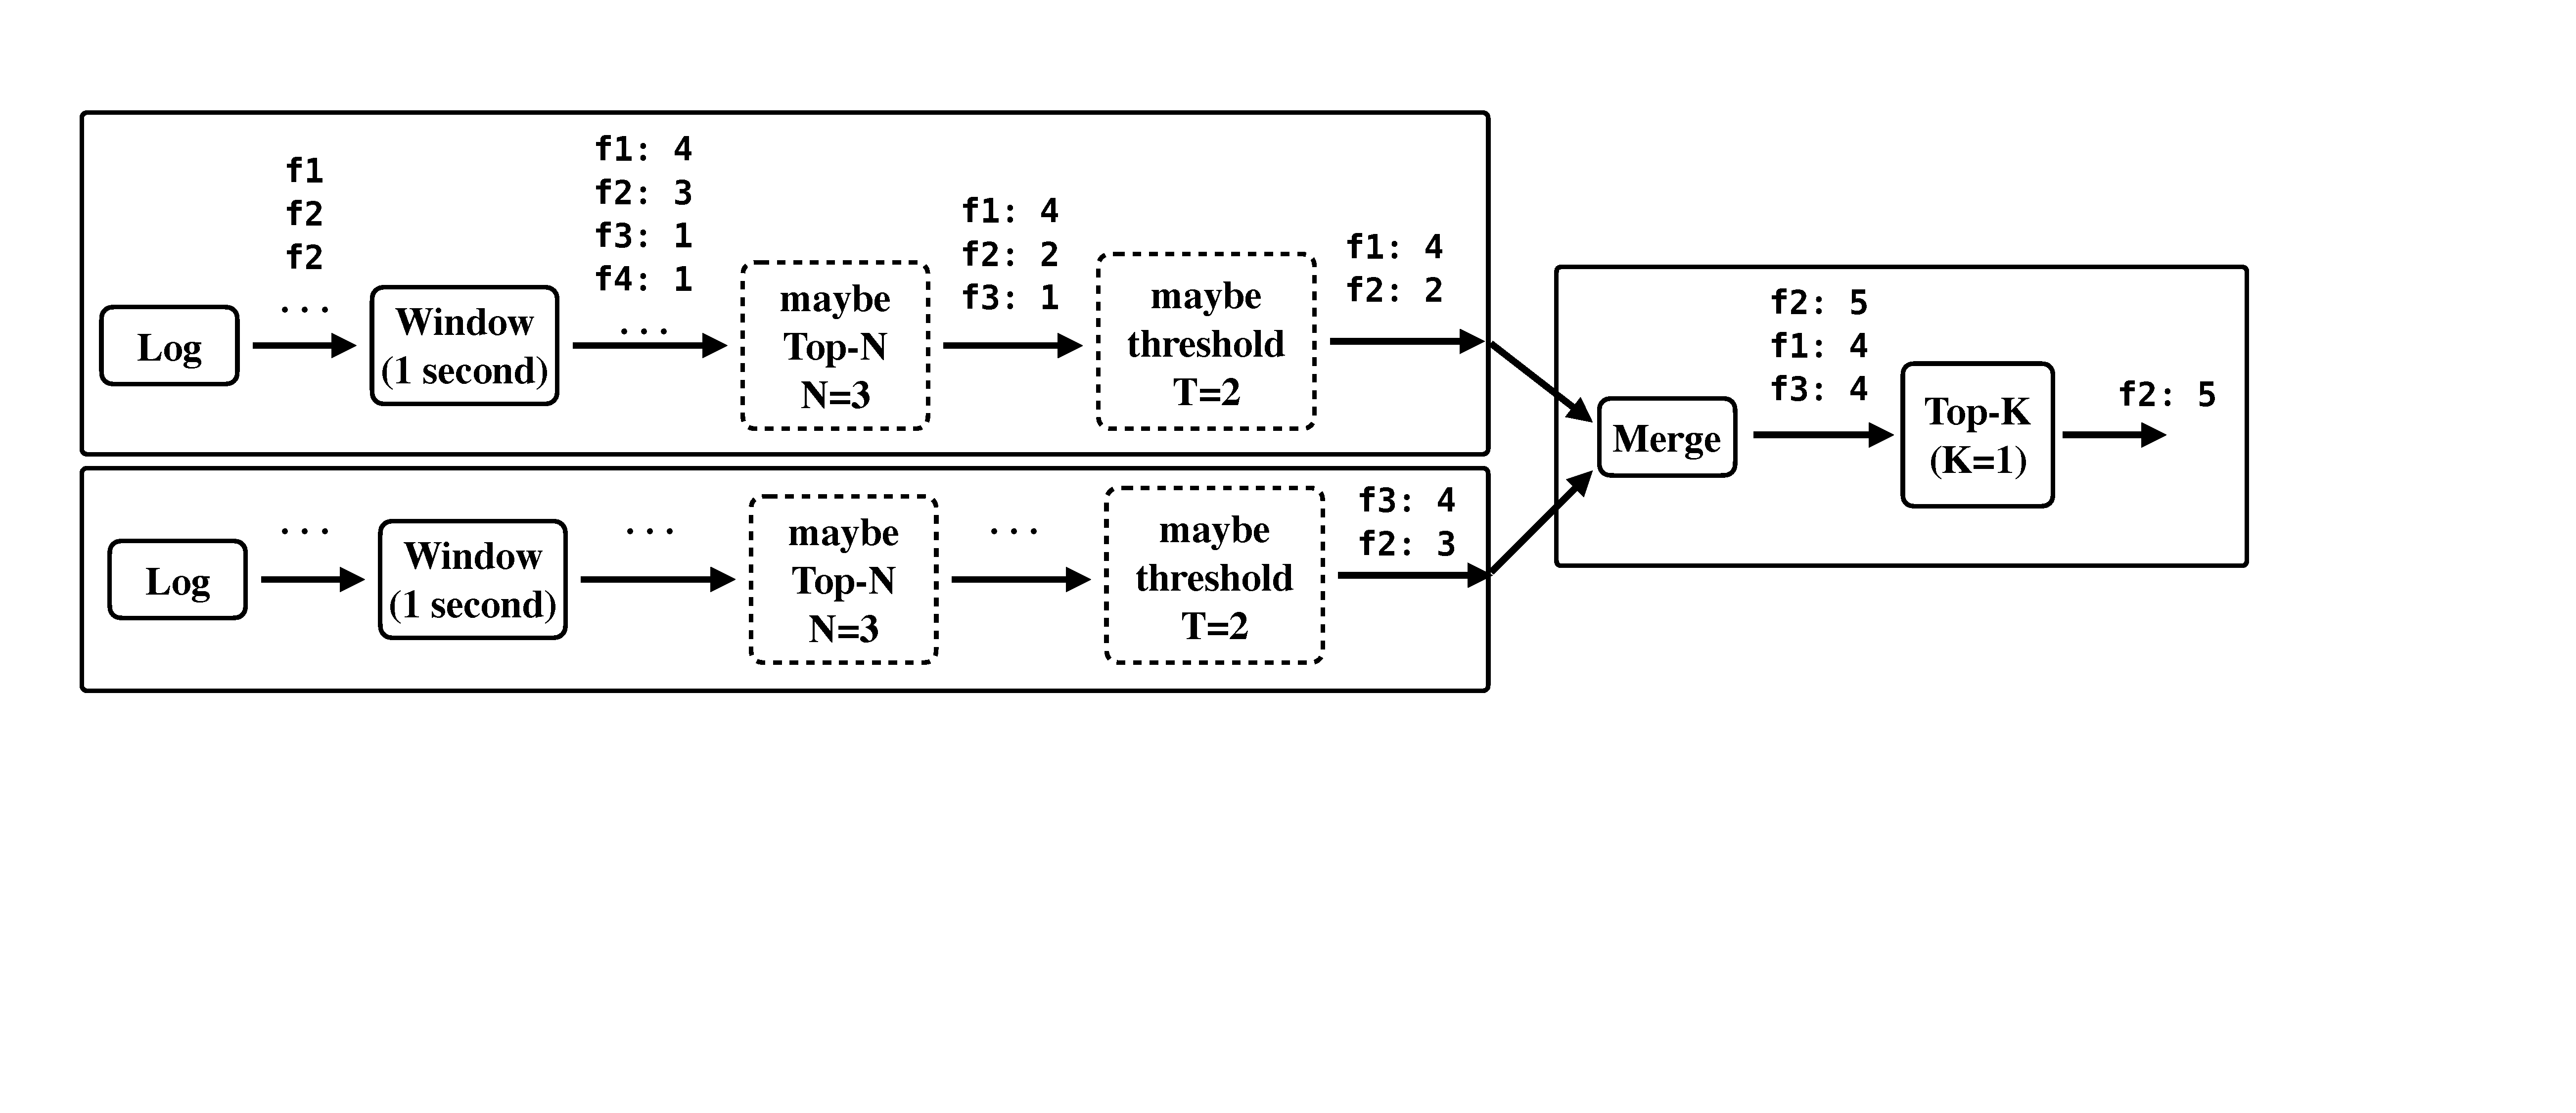
\includegraphics[width=\columnwidth]{figures/topk.pdf}
  \caption{A distributed Top-K application with two degradation operations:
    \texttt{head} and \texttt{threshold}. In this example, \texttt{f2}, which is
    not in Top-1 for either client, becomes the global Top-1 after the merge. It
    would have been purged if the clients use threshold T=3, demonstrating
    degradation that reduces data sizes affects fidelity.}
  \label{fig:topk}
\end{figure}

\para{Distributed Top-K.} This application aggregates machine logs from
geo-distributed servers to find out the Top-K most accessed files, similar to
many Top-K queries~\cite{babcock2003distributed}.

\autoref{fig:topk} illustrates our processing pipeline with two degradation
operations. First each source node summarizes the log using \texttt{Window}
operator to reduce the data size, a pre-processing step. As many real-world
access patterns follow a long tail distribution, there can be a
large-but-irrelevant tail that contributes little to the final Top-K. Each
source node then filters the tail: (1) head(\texttt{N}) takes the top \texttt{N}
entries; (2) threshold(\texttt{T}) filters small entries whose count is smaller
than \texttt{T}. These two operations affect the final result and the exact
impact depends on data distribution. We implement these two operators by using
\sysname{}'s \maybe{} abstraction.

To measure the accuracy, we need to compare the correlation between two ranked
list. Kendall's~$\tau$~\cite{abdi2007kendall} is a correlation measure of the
concordance between two ranked list. The output ranges from \(-1\) to 1,
representing no agreement to complete agreement. To integrate with \sysname{},
we convert Kendall's~$\tau$ to [0, 1] with a linear transformation. For our
evaluation, we set K as 50 and use Apache log files that record and store user
access statistics for the \href{https://www.sec.gov}{SEC.gov} website. The logs
are split into four groups, simulating four geo-distributed nodes monitoring web
accesses. To match the load of popular web servers, we compress one hour's logs
into one second.

%%% Local Variables:
%%% mode: latex
%%% TeX-master: "../network"
%%% End:

%% LocalWords: runtime dataset quantization geo
